\chapter{Appendix}
\blindtext

\section{…} % TODO
\begin{figure}
  \centering
  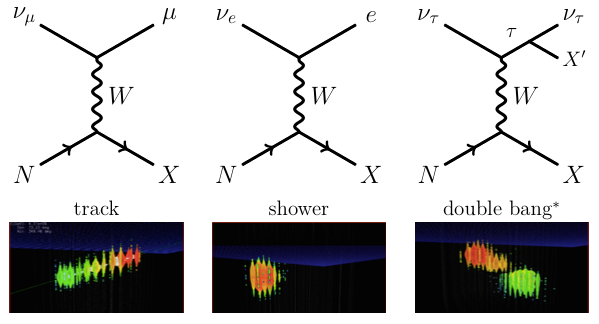
\includegraphics[width=\textwidth]{content/img/flavors1.png}
  \caption{
    Shapes of the Cherenkov light produced by neutrinos of different flavors.
    \citationneeded{}
  }
  \label{fig:img:icecube:interactions}
\end{figure}


\section{\dseaplus{}: Complete algorithm} \label{sec:alg:dseaplus}
\begin{algorithm}
  \caption{
    The \dseaplus{} algorithm with reweighting of training examples and adjustable stepsize. \cite{dsea_mirko}
    \todo[inline]{
      This is taken 1:1 from Mirko's thesis.
      I didn't quite get @Karolin's feedback on this:
      Should I remove it?
      }
    }
  \label{alg:dseaplus}
  \begin{algorithmic}
    \newcommand{\f}{\mathbf{f}}
    \newcommand{\hatf}{\hat{\mathbf{f}}}
    \newcommand{\x}{\mathbf{x}}

    \Require{
      \\
      Observed data set $\mathcal{D}_\text{obs} = \{ \x_n \in \mathcal{X} : 1 \leq n \leq N \}$ \\
      Training data set $\mathcal{D}_\text{test} = \{ (\x_n, y_n) \in \mathcal{X} \times \{1,\ldots,I\} : 1 \leq n \leq N' \}$ \\
      $\tau \geq 0$, regularization strength employed in the stepsize adaptation (default: \num{0}) \\
      $\epsilon > 0$, the minimal $\chi_\text{Sym}^2$ distance between subsequent iterations (default: \num{E-6}) \\
      Prior density $\hatf^{(0)}$ (default: $\hatf_i^{(0)} = \frac{1}{I} \forall 1 \leq j \leq J$)
    }
    \Ensure Estimated target density $\hatf \in \mathbb{R}^I$
    \State $k \gets 0$
    \Repeat
      \State $k \gets k-1$\;
      \State $\forall 1 \leq n \leq N': w_n^{(k)} \gets \hatf_{i (n)}^{(k-1)} / \f_{i (n)}^t$\;
      \State Infer $\mathcal{M}$ from $\mathcal{D}_\text{train}$ weighted by $w_n^{(k)+}$\;
      \State $\forall 1 \leq i \leq I: p_i^{(k)} \gets \frac{1}{N} \sum_{n=1}^N c_{\mathcal{M}}(i|\x_n) - \hatf^{(k-1)}$\;
      \State $\alpha_{\textsc{Run}}^{(k)} \gets \operatorname{argmin}_{\alpha \geq 0} \ell_r(\hatf^{(k-1)} + \alpha p^{(k)})$\;
      \State $\hatf_i^{(k)+} \gets \hatf^{(k-1)} + \alpha_{\textsc{Run}}^{(k)} \cdot p^{(k)}$\;
    \Until $\chi_\text{Sym}^2(\hatf^{(k)}, \hatf^{(k-1)}) \leq \epsilon$\; \\
    \Return $\hatf \gets \hatf^{(k)}$
  \end{algorithmic}
\end{algorithm}



\section{From threshold to per-class probabilities}
\label{sec:appendix:corn_probas}
% NOTE: Keep the $q$-notation from the CORN paper/section!
\blindtext


\section{Adding support for weighting}
\label{sec:appendix:corn_weighting}
% TODO: Reference this section in the main text
\begin{minted}{python}
  loss = -torch.sum(
    (F.logsigmoid(pred)*train_labels
      + (F.logsigmoid(pred) - pred)*(1-train_labels))
    * train_weights # ← new
  )
\end{minted}


\section{Dataset}
\begin{figure}
  \centering
  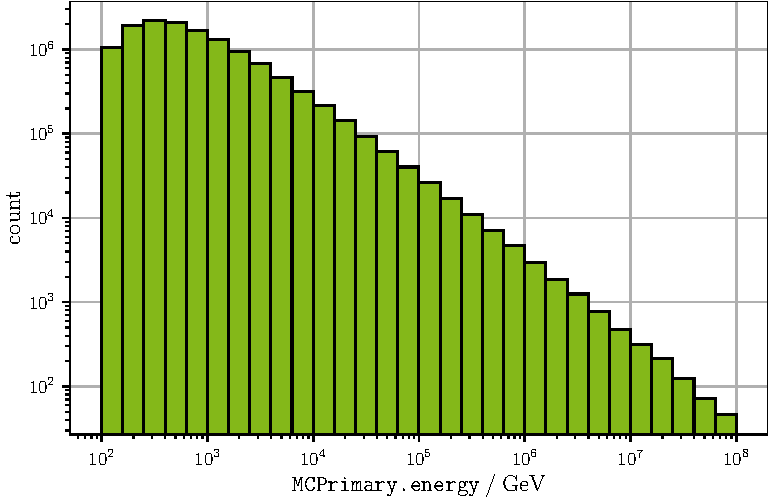
\includegraphics[scale=1]{content/plots/dataset:raw:histogram_full.pdf}
  \caption{Energy spectrum of the full, untouched Monte-Carlo dataset using 30 bins.}
  % TODO: Actually the full? Maybe I used only 1 million, which would mess up the y axis.
  \label{fig:dataset:raw:histogram}
\end{figure}

% TODO: Add a table of all features?

\section{Bootstrap distributions}
\begin{figure}
  \centering
  % TODO: correct dimensions
  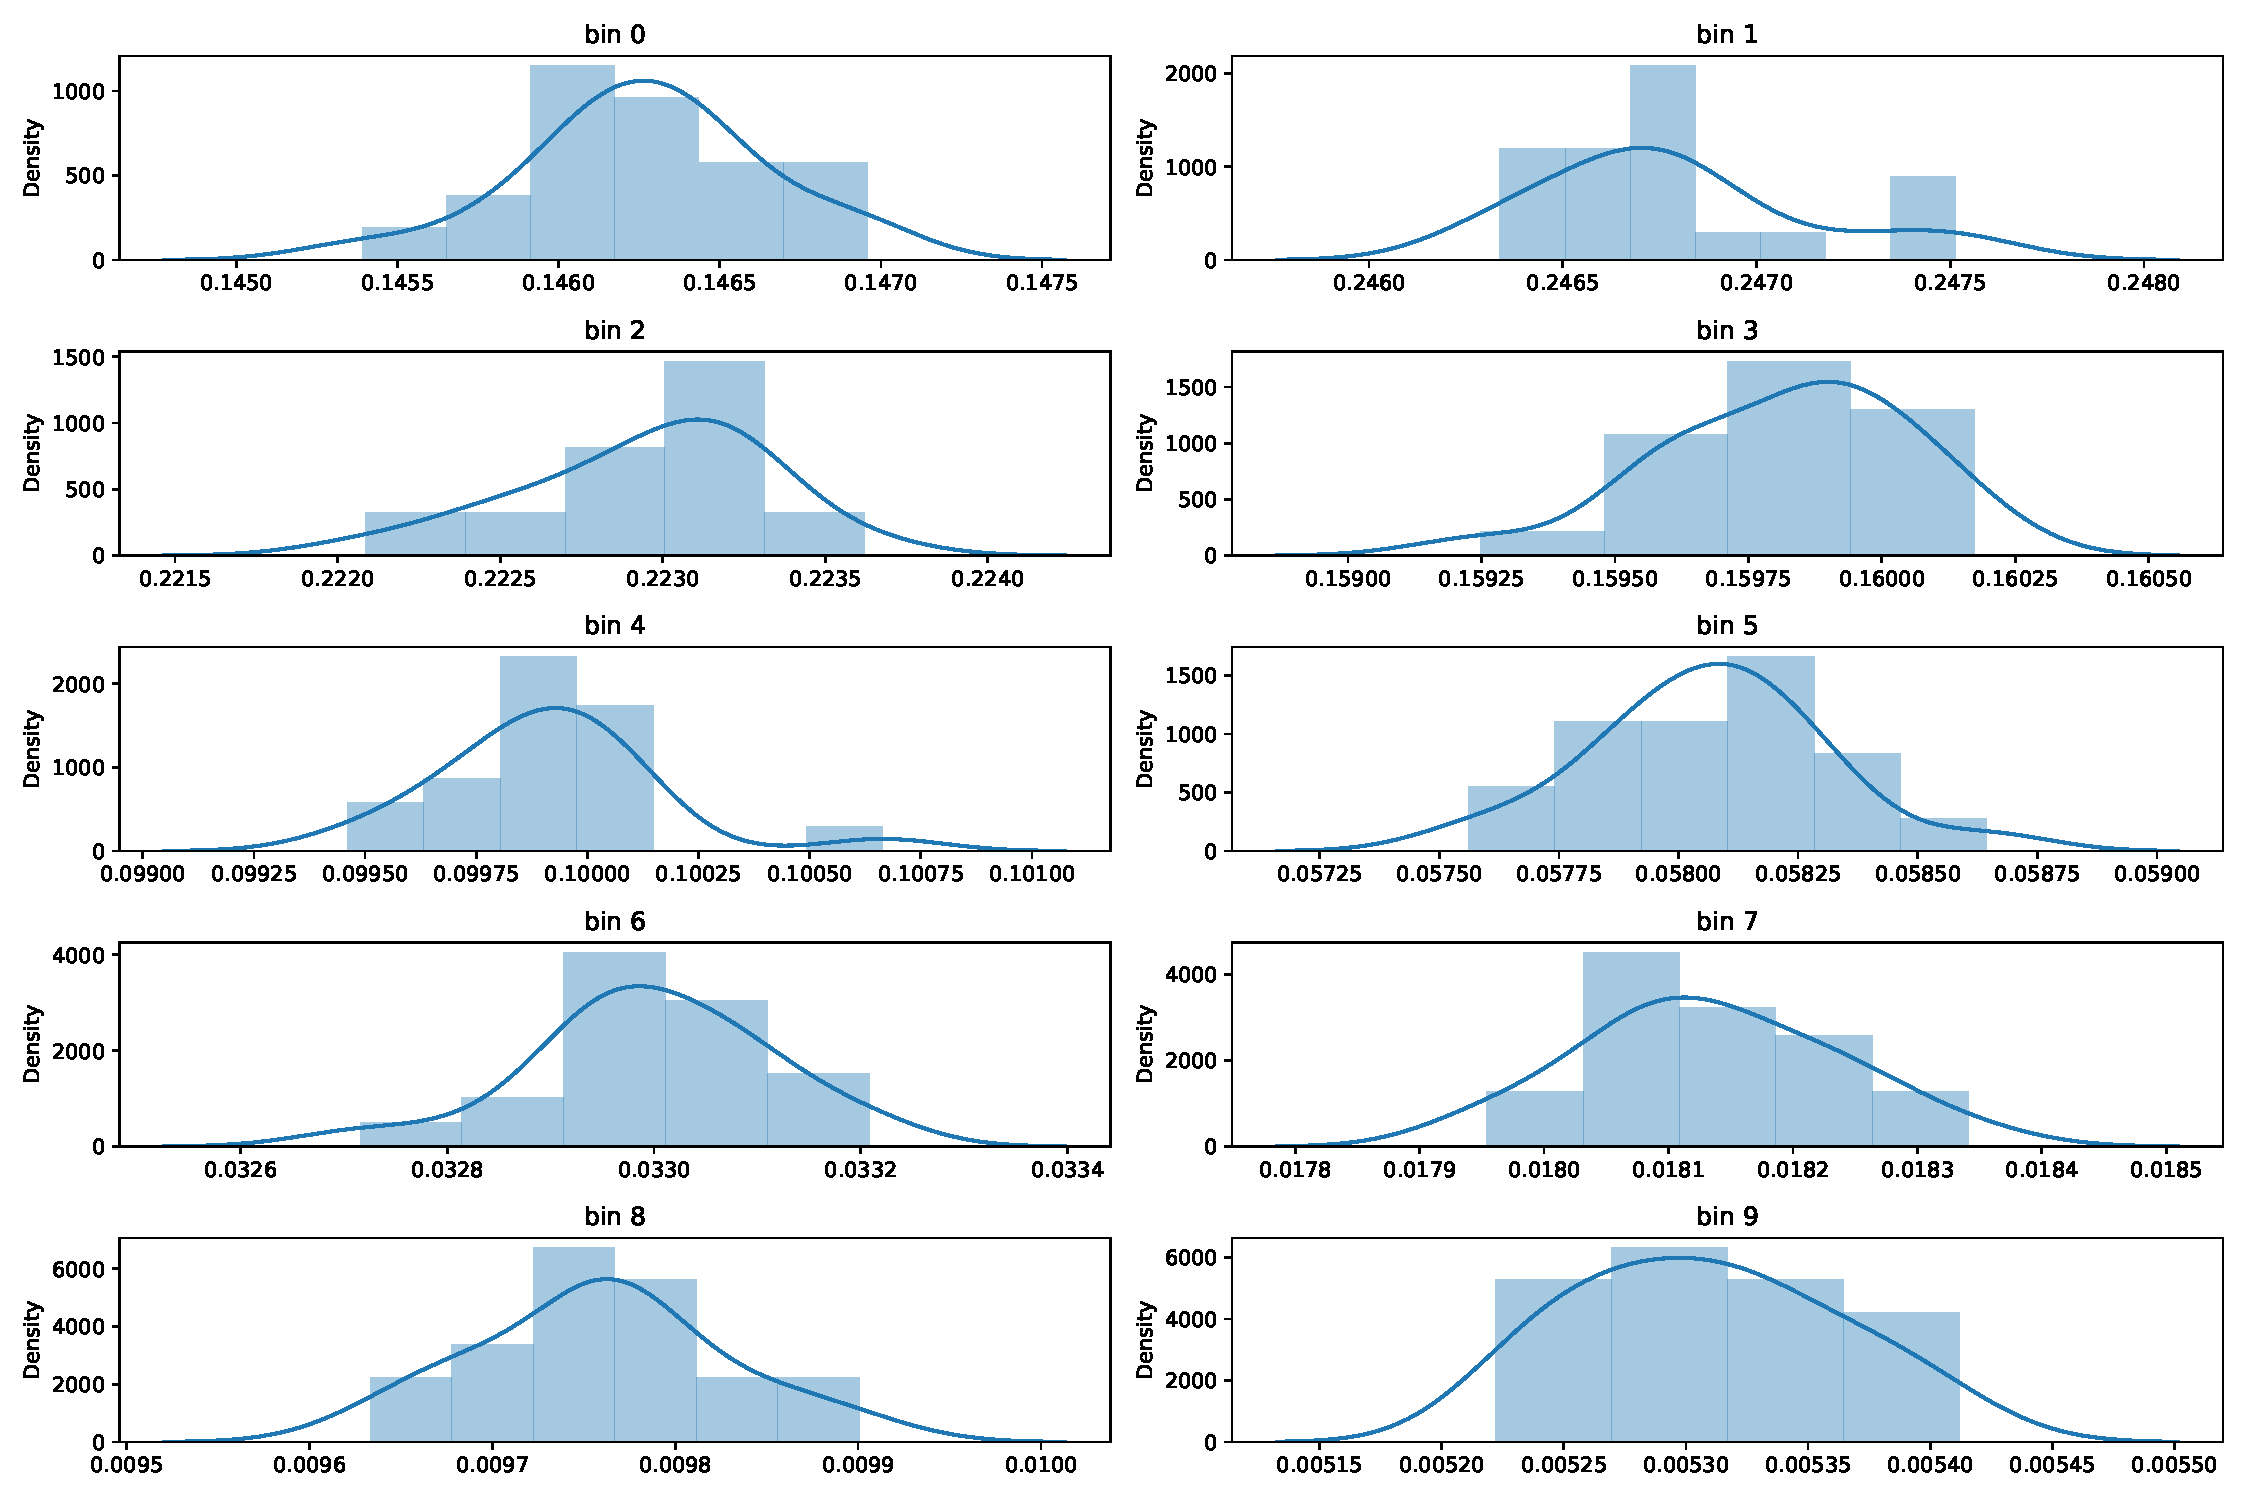
\includegraphics[width=\textwidth]{content/plots/halftime/bootstrap_distributions.pdf}
  \caption{Bootstrap distributions TODO.}
  \label{fig:bootstrap:distributions}
\end{figure}


\section{Links etc.}
\begin{description}
  \item[Dataset in the chair's \texttt{POOL} file system] \texttt{/net/big-tank/POOL/users/lkardum/new\_mc\_binning.csv} (\SI{14.6}{\giga\byte})
  % https://git.e5.physik.tu-dortmund.de/shaefs/bachelor_thesis/
  % https://git.e5.physik.tu-dortmund.de/nweitkemper/ba % TODO: move master → main
\end{description}
% TODO: Link to GitHub / GitLab / code on Phobos
